\documentclass[aspectratio=169]{beamer}

\usetheme{Madrid}
\usecolortheme{seahorse}
\setbeamertemplate{navigation symbols}{}
\setbeamertemplate{footline}[frame number]

\usepackage{graphicx}
\usepackage{booktabs}
\usepackage{amsmath}
\usepackage{listings}
\usepackage{hyperref}

\lstset{
  basicstyle=\ttfamily\tiny,
  breaklines=true,
  frame=single,
  columns=fullflexible
}

\title[Parallel TSP]{Parallel Travelling Salesman Problem Solver}
\subtitle{Island-Model Genetic Algorithm with MPI}
\author{Parallel Programming Project}
\date{June 2026}

\begin{document}

% 1
\begin{frame}
  \titlepage
\end{frame}

% 2
\begin{frame}{Project Goal}
  \begin{itemize}
    \item Solve the Travelling Salesman Problem with a heuristic method.
    \item Parallelize the search with MPI on a multi-node cluster.
    \item Measure correctness, input-size behavior, granularity, load balance, and speedup.
    \item Keep the solver in C++; use Python only for visualization and plotting.
  \end{itemize}
\end{frame}

% 3
\begin{frame}{Travelling Salesman Problem}
  \begin{itemize}
    \item Input: $N$ cities with 2D coordinates.
    \item Output: one closed tour visiting every city exactly once.
    \item Objective: minimize total Euclidean route length.
  \end{itemize}
  \[
    L(T) = \sum_{i=0}^{N-1} d(t_i, t_{(i+1) \bmod N})
  \]
  \begin{block}{Reason for heuristic search}
    TSP is NP-hard; exact brute force is only practical for very small $N$.
  \end{block}
\end{frame}

% 4
\begin{frame}{Repository Layout}
  \begin{tabular}{ll}
    \toprule
    Folder & Purpose \\
    \midrule
    \texttt{cpp/} & GA core, local search, MPI solver, tests \\
    \texttt{python/} & visualization, validation, experiments \\
    \texttt{data/} & city coordinate files and generator \\
    \texttt{cluster/} & OpenMPI, SSH, sync, launch scripts \\
    \texttt{results/} & CSV files, figures, generated outputs \\
    \texttt{report/} & report and presentation files \\
    \bottomrule
  \end{tabular}
\end{frame}

% 5
\begin{frame}{Main C++ Components}
  \begin{itemize}
    \item \texttt{ga\_core.hpp}: distance matrix, tour length, selection, OX crossover, mutation.
    \item \texttt{local\_search.hpp}: 2-opt, Or-opt, optional memetic polish.
    \item \texttt{tsp\_island.cpp}: MPI island-model solver.
    \item \texttt{tsp\_sequential.cpp}: sequential baseline.
    \item \texttt{test\_*.cpp}: unit tests for operators and local search.
  \end{itemize}
\end{frame}

% 6
\begin{frame}{Tour Representation}
  \begin{itemize}
    \item One individual is a permutation of city indices.
    \item Example for 6 cities: \texttt{[3, 0, 5, 1, 4, 2]}.
    \item The last city connects back to the first city.
    \item A valid tour must contain each index exactly once.
  \end{itemize}
  \begin{block}{Fitness}
    The fitness value is total tour length; smaller is better.
  \end{block}
\end{frame}

% 7
\begin{frame}{Sequential GA Baseline}
  \begin{enumerate}
    \item Generate an initial population of random tours.
    \item Evaluate all tour lengths.
    \item Keep the best individual by elitism.
    \item Select parents by tournament selection.
    \item Create children with order crossover.
    \item Apply swap and segment-reversal mutation.
    \item Repeat for a fixed number of generations.
  \end{enumerate}
\end{frame}

% 8
\begin{frame}{Genetic Operators}
  \begin{itemize}
    \item Tournament selection: choose the best among $k=5$ sampled individuals.
    \item Order crossover: preserve a segment from one parent and fill the rest using the order of another parent.
    \item Mutation:
      \begin{itemize}
        \item random city swap,
        \item random segment reversal.
      \end{itemize}
    \item Elitism: copy the best local tour into the next generation.
  \end{itemize}
\end{frame}

% 9
\begin{frame}{Local Search}
  \begin{itemize}
    \item Optional memetic step controlled by \texttt{--twoopt}.
    \item 2-opt removes edge crossings by reversing a segment.
    \item Or-opt moves a short segment to a better insertion position.
    \item Applied only periodically to the best local individual to limit cost.
  \end{itemize}
\end{frame}

% 10
\begin{frame}{Parallelism Level}
  \begin{block}{Level}
    Coarse-grained task-level parallelism.
  \end{block}
  \begin{itemize}
    \item Each MPI rank runs one independent GA population.
    \item The city data and distance matrix are replicated on every rank.
    \item Different ranks use different random seeds and explore different regions.
  \end{itemize}
  \begin{block}{Decomposition}
    Hybrid task and exploratory decomposition.
  \end{block}
\end{frame}

% 11
\begin{frame}{Why Exploratory Decomposition?}
  \begin{itemize}
    \item A TSP tour is a global permutation, so splitting cities directly is not natural.
    \item GA search is stochastic; multiple populations can search different areas.
    \item Islands can run mostly independently and communicate only occasionally.
    \item This creates coarse granularity and reduces communication frequency.
  \end{itemize}
\end{frame}

% 12
\begin{frame}{Process Mapping}
  \begin{itemize}
    \item One-dimensional mapping:
  \end{itemize}
  \[
    \text{MPI rank } r \rightarrow \text{island } r
  \]
  \begin{itemize}
    \item Each rank owns one population and its fitness array.
    \item Cluster hostfile maps ranks round-robin across four machines.
    \item Up to 48 ranks were used, limited by the common physical-core count.
  \end{itemize}
\end{frame}

% 13
\begin{frame}{Communication Strategy}
  \begin{itemize}
    \item Periodic blocking collective communication.
    \item Every \texttt{--sync} generations:
      \begin{enumerate}
        \item each rank finds its local best,
        \item \texttt{MPI\_Allreduce(MINLOC)} finds the global best and owner,
        \item owner broadcasts the best tour with \texttt{MPI\_Bcast},
        \item other ranks partially migrate this information into local populations.
      \end{enumerate}
    \item Logical topology: global collective, not ring and not master-slave.
  \end{itemize}
\end{frame}

% 14
\begin{frame}{Partial Global-Best Migration}
  \begin{itemize}
    \item The owner broadcasts the best tour.
    \item Other islands do not clone the full tour.
    \item They use OX crossover between:
      \begin{itemize}
        \item the global best tour,
        \item a random local mate.
      \end{itemize}
    \item The child replaces one of the worst local individuals.
    \item Goal: spread good sub-routes while preserving diversity.
  \end{itemize}
\end{frame}

% 15
\begin{frame}{Parallel Algorithm}
\begin{lstlisting}
Initialize MPI
Read cities and build distance matrix on every rank
Create one random population per rank

for each generation:
    evolve local population
    optionally polish local best

    if generation is a sync point:
        local_best = best local tour
        global_best, owner = MPI_Allreduce(MINLOC)
        owner broadcasts global_best tour
        non-owner ranks inject partial migrants
        update convergence-stop state

Gather final global best and write outputs
Finalize MPI
\end{lstlisting}
\end{frame}

% 16
\begin{frame}{Load Balancing}
  \begin{itemize}
    \item Default: same population size on every rank.
    \item This gives approximately equal compute work per rank.
    \item The cluster run limits ranks per machine by the weakest machine.
    \item Optional \texttt{--auto-balance} benchmarks local speed and gives faster ranks larger populations.
  \end{itemize}
  \begin{block}{Granularity}
    One GA population per process: coarse enough to avoid per-generation communication.
  \end{block}
\end{frame}

% 17
\begin{frame}{Instrumentation}
  \begin{itemize}
    \item \texttt{comm\_s}: measured time inside MPI calls.
    \item \texttt{compute\_s}: estimated as total time minus communication time.
    \item \texttt{makespan\_s}: maximum elapsed time over all ranks.
    \item \texttt{--stats}: writes one CSV row per rank.
    \item \texttt{--out}: writes final tour and convergence history.
    \item \texttt{--live}: streams JSONL for real-time visualization.
  \end{itemize}
\end{frame}

% 18
\begin{frame}{Correctness Validation}
  \begin{itemize}
    \item Unit tests verify:
      \begin{itemize}
        \item distance matrix correctness,
        \item OX crossover produces valid permutations,
        \item mutation preserves permutations,
        \item local search does not worsen tours.
      \end{itemize}
    \item \texttt{validate\_tour.py} independently recomputes route length.
    \item For $N \le 10$, brute force gives the exact optimum for comparison.
  \end{itemize}
\end{frame}

% 19
\begin{frame}{Cluster Setup}
  \begin{itemize}
    \item Four machines connected over a LAN.
    \item OpenMPI 5.0.9 pinned at \texttt{/opt/openmpi-5.0.9}.
    \item Password-less SSH for remote rank launch.
    \item Same repository path on every node.
    \item Launcher uses \texttt{--map-by seq --bind-to none} for heterogeneous nodes.
  \end{itemize}
\end{frame}

% 20
\begin{frame}{Experiment 1: Runtime vs Input Size}
  \begin{figure}
    \centering
    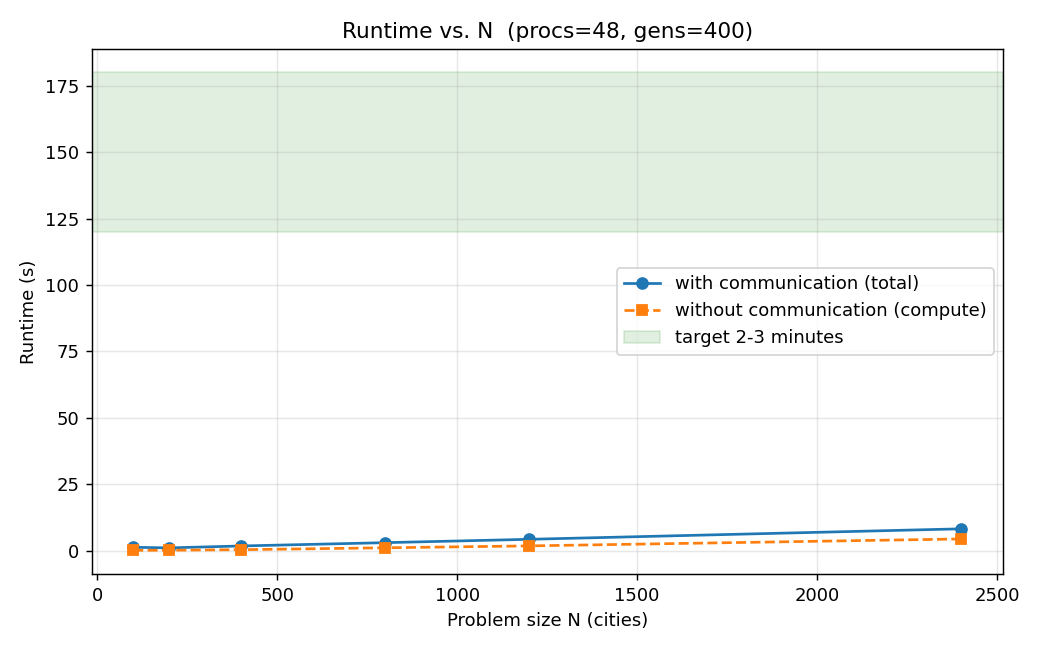
\includegraphics[width=0.78\linewidth]{../results/exp_size.png}
  \end{figure}
  \vspace{-0.3cm}
  \small Initial 400-generation sweep used to study growth trend.
\end{frame}

% 21
\begin{frame}{Final N* Selection}
  \begin{table}
  \centering
  \small
  \begin{tabular}{rrrr}
  \toprule
  $N$ & Total (s) & Comm (s) & Compute (s) \\
  \midrule
  1200 & 54.54 & 25.90 & 28.65 \\
  1800 & 86.99 & 34.33 & 52.66 \\
  2400 & 154.27 & 64.05 & 90.22 \\
  \bottomrule
  \end{tabular}
  \end{table}
  \begin{itemize}
    \item Final choice: $N^*=2400$, \texttt{gens*=10500}, 48 ranks.
    \item Official repeated run: 145.97s, inside the 120--180s target.
  \end{itemize}
\end{frame}

% 22
\begin{frame}{Experiment 2: Granularity}
  \begin{figure}
    \centering
    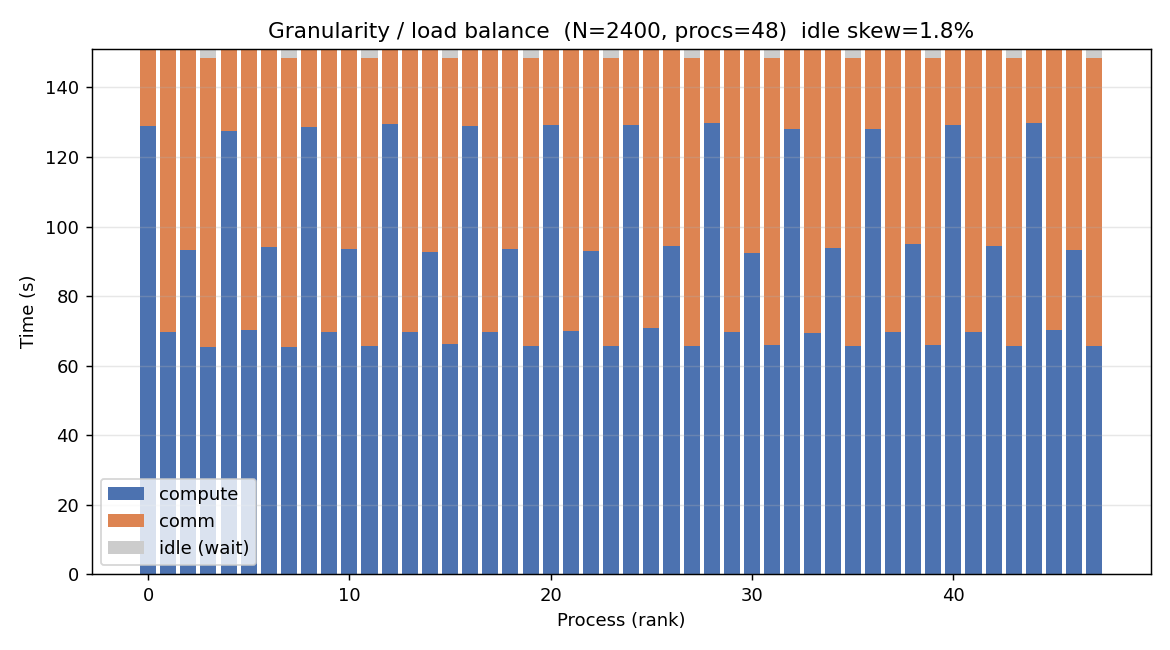
\includegraphics[width=0.82\linewidth]{../results/exp_gran.png}
  \end{figure}
\end{frame}

% 23
\begin{frame}{Granularity Result}
  \begin{itemize}
    \item Run configuration: $N^*=2400$, \texttt{gens=10500}, 48 ranks.
    \item Each rank owns one island population.
    \item The measured idle skew is about 1.8\%.
    \item This is below the 25\% imbalance threshold.
  \end{itemize}
  \begin{block}{Conclusion}
    The workload is balanced for this configuration.
  \end{block}
\end{frame}

% 24
\begin{frame}{Experiment 3: Speedup}
  \begin{figure}
    \centering
    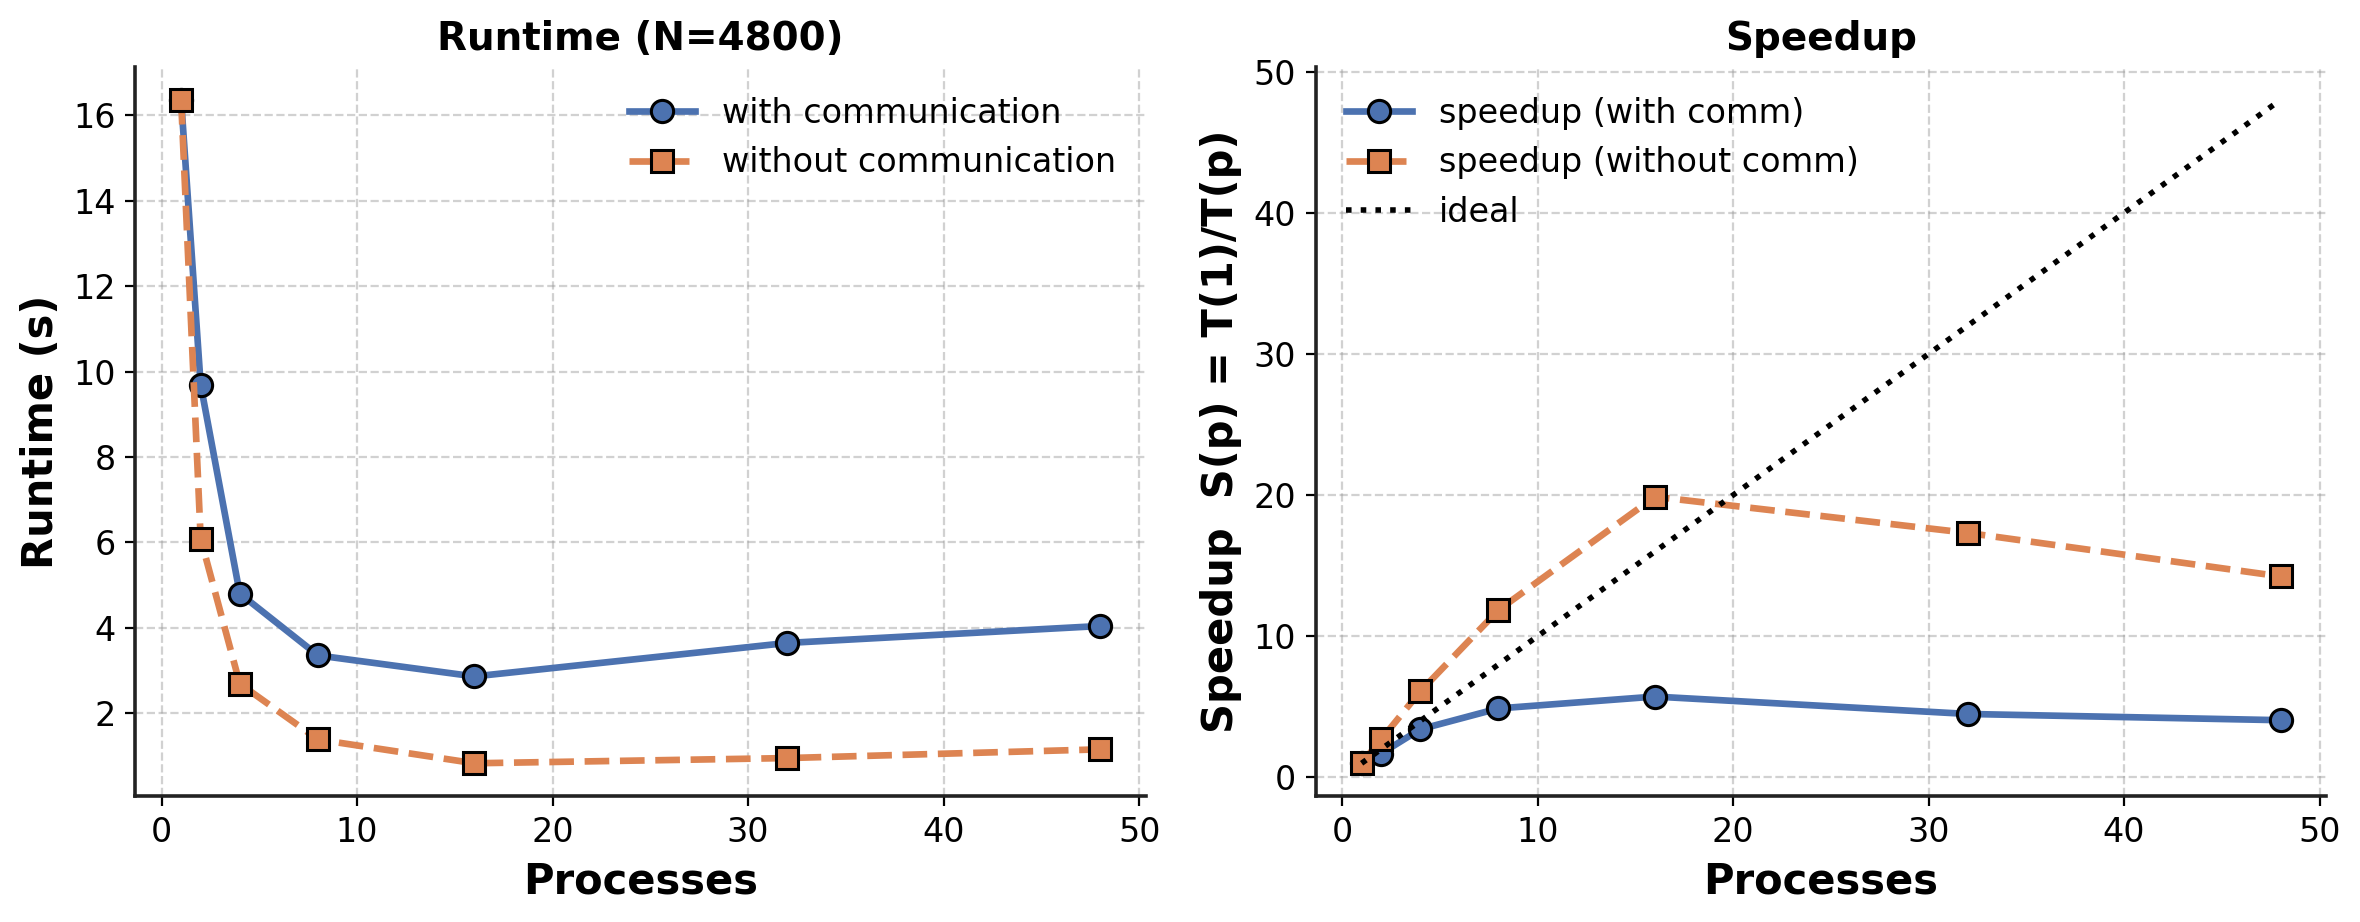
\includegraphics[width=0.82\linewidth]{../results/exp_speedup.png}
  \end{figure}
\end{frame}

% 25
\begin{frame}{Speedup Result and Conclusion}
  \begin{itemize}
    \item Speedup experiment uses $2N^*=4800$ cities and fixed total population.
    \item Speedup improves up to 16 processes, then decreases.
    \item No-communication speedup is much higher than total speedup.
    \item The GA computation scales, but repeated collective communication dominates at high process counts.
    \item The island model is correct and balanced, but large process counts require larger problem sizes or less frequent synchronization.
  \end{itemize}
  \begin{block}{Final Summary}
    Parallel level: task/exploratory. Mapping: 1D rank-to-island. Communication: blocking MPI collectives. Load balance: acceptable in the measured run.
  \end{block}
\end{frame}

\end{document}
